\section{Object3D Class Reference}
\label{classObject3D}\index{Object3D@{Object3D}}
{\tt \#include $<$object3d.h$>$}

Inheritance diagram for Object3D::\begin{figure}[H]
\begin{center}
\leavevmode
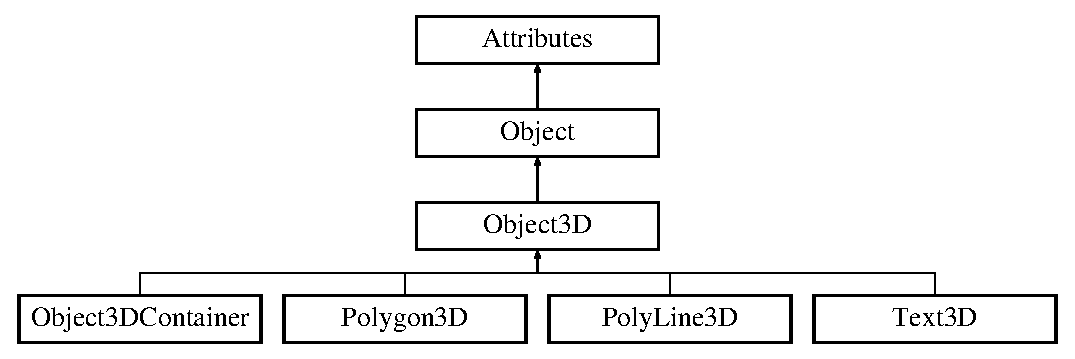
\includegraphics[height=4cm]{classObject3D}
\end{center}
\end{figure}
\subsection*{Public Methods}
\begin{CompactItemize}
\item 
virtual std::pair$<$ double, double $>$ {\bf get\-Depth\-Range} ()=0
\item 
virtual void {\bf render} ({\bf Figure} $\ast$, double x\-Offset, double y\-Offset, double scale, double distance, double min\-Depth, double max\-Depth, int min\-Fig\-Depth=0, int max\-Fig\-Depth=999)=0
\item 
virtual void {\bf apply\-Matrix} ({\bf Matrix}$<$ double $>$ $\ast$)=0
\item 
virtual void {\bf translate} ({\bf Coordinate3D} $\ast$)=0
\end{CompactItemize}


\subsection{Member Function Documentation}
\index{Object3D@{Object3D}!applyMatrix@{applyMatrix}}
\index{applyMatrix@{applyMatrix}!Object3D@{Object3D}}
\subsubsection{\setlength{\rightskip}{0pt plus 5cm}virtual void Object3D::apply\-Matrix ({\bf Matrix}$<$ double $>$ $\ast$)\hspace{0.3cm}{\tt  [pure virtual]}}\label{classObject3D_a2}




Implemented in {\bf Object3DContainer} {\rm (p.\,\pageref{classObject3DContainer_a2})}, {\bf Polygon3D} {\rm (p.\,\pageref{classPolygon3D_a6})}, {\bf Poly\-Line3D} {\rm (p.\,\pageref{classPolyLine3D_a5})}, and {\bf Text3D} {\rm (p.\,\pageref{classText3D_a7})}.\index{Object3D@{Object3D}!getDepthRange@{getDepthRange}}
\index{getDepthRange@{getDepthRange}!Object3D@{Object3D}}
\subsubsection{\setlength{\rightskip}{0pt plus 5cm}virtual std::pair$<$ double, double$>$ Object3D::get\-Depth\-Range ()\hspace{0.3cm}{\tt  [pure virtual]}}\label{classObject3D_a0}




Implemented in {\bf Object3DContainer} {\rm (p.\,\pageref{classObject3DContainer_a0})}, {\bf Polygon3D} {\rm (p.\,\pageref{classPolygon3D_a4})}, {\bf Poly\-Line3D} {\rm (p.\,\pageref{classPolyLine3D_a4})}, and {\bf Text3D} {\rm (p.\,\pageref{classText3D_a5})}.\index{Object3D@{Object3D}!render@{render}}
\index{render@{render}!Object3D@{Object3D}}
\subsubsection{\setlength{\rightskip}{0pt plus 5cm}virtual void Object3D::render ({\bf Figure} $\ast$, double {\em x\-Offset}, double {\em y\-Offset}, double {\em scale}, double {\em distance}, double {\em min\-Depth}, double {\em max\-Depth}, int {\em min\-Fig\-Depth} = 0, int {\em max\-Fig\-Depth} = 999)\hspace{0.3cm}{\tt  [pure virtual]}}\label{classObject3D_a1}




Implemented in {\bf Object3DContainer} {\rm (p.\,\pageref{classObject3DContainer_a1})}, {\bf Polygon3D} {\rm (p.\,\pageref{classPolygon3D_a5})}, {\bf Poly\-Line3D} {\rm (p.\,\pageref{classPolyLine3D_a6})}, and {\bf Text3D} {\rm (p.\,\pageref{classText3D_a6})}.\index{Object3D@{Object3D}!translate@{translate}}
\index{translate@{translate}!Object3D@{Object3D}}
\subsubsection{\setlength{\rightskip}{0pt plus 5cm}virtual void Object3D::translate ({\bf Coordinate3D} $\ast$)\hspace{0.3cm}{\tt  [pure virtual]}}\label{classObject3D_a3}




Implemented in {\bf Object3DContainer} {\rm (p.\,\pageref{classObject3DContainer_a3})}, {\bf Polygon3D} {\rm (p.\,\pageref{classPolygon3D_a7})}, {\bf Poly\-Line3D} {\rm (p.\,\pageref{classPolyLine3D_a7})}, and {\bf Text3D} {\rm (p.\,\pageref{classText3D_a8})}.

The documentation for this class was generated from the following file:\begin{CompactItemize}
\item 
{\bf object3d.h}\end{CompactItemize}
